% \begin{figure*}[h]
%   \begin{center}
%     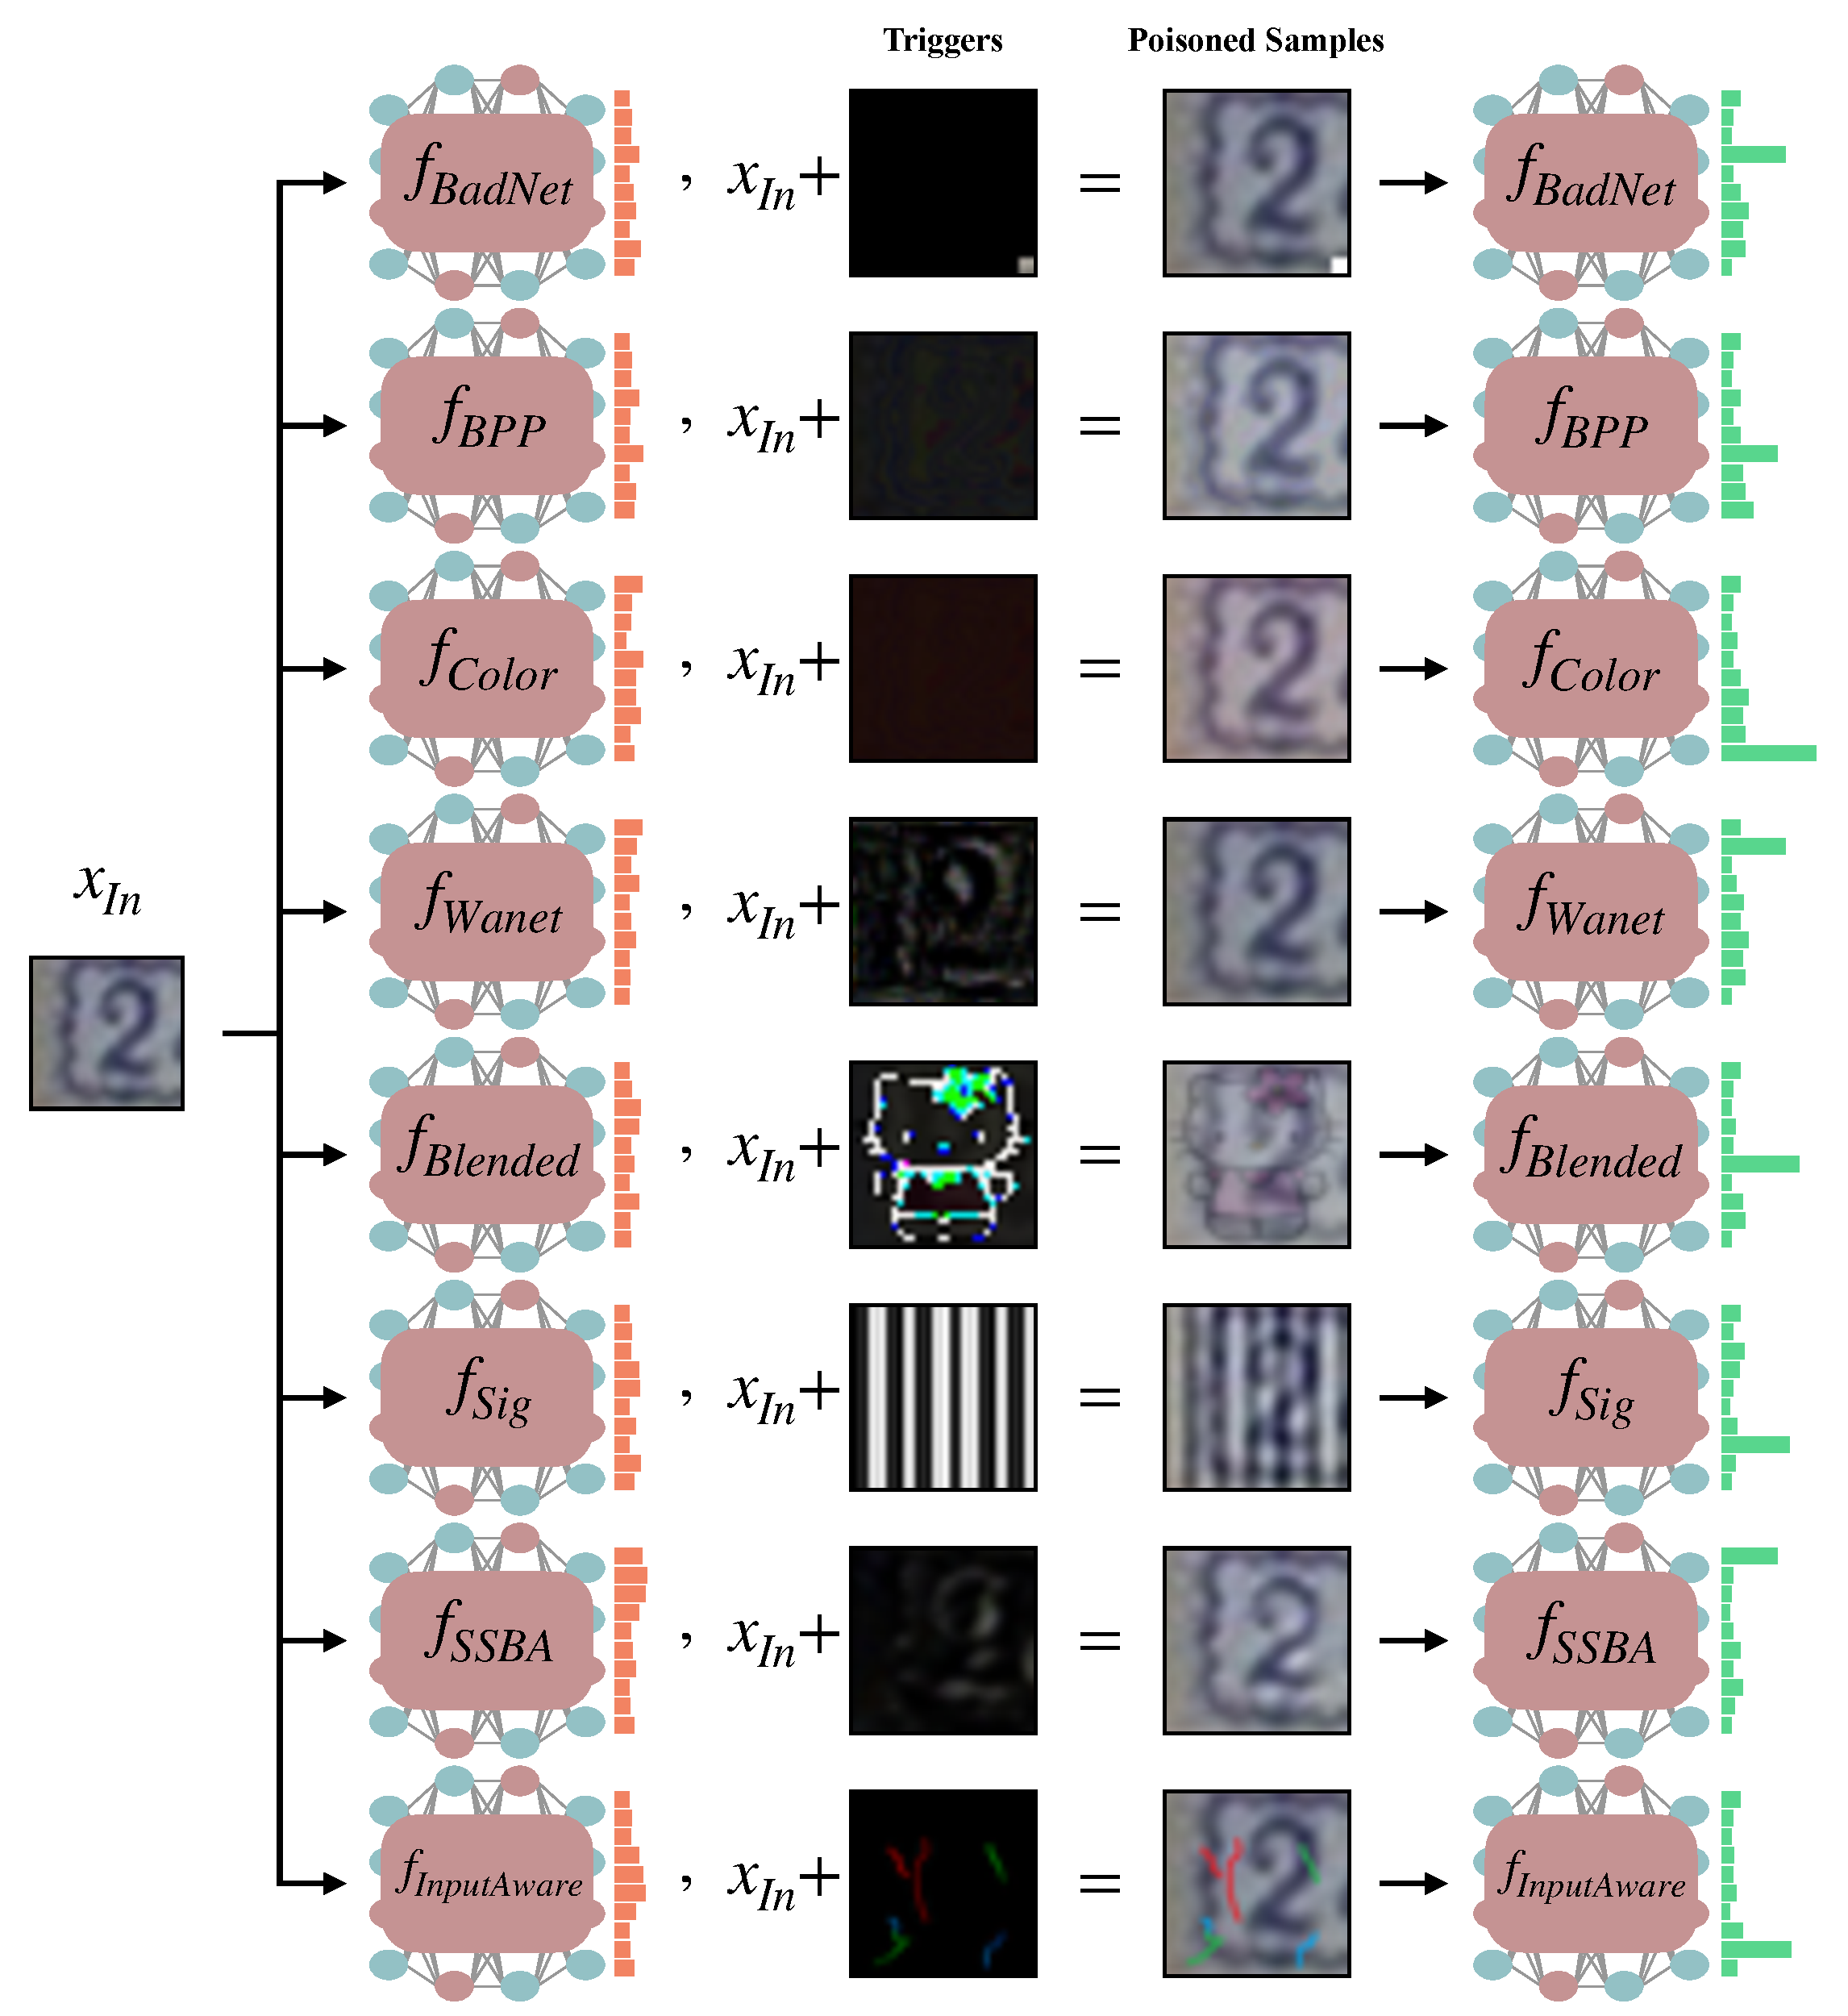
\includegraphics[width=1\linewidth, bb=0 0 1100 1200]{Images/TriggerOnOOD.pdf}
%     \caption{The effect of overlaying triggers on OOD data, in various attacks. As demonstrated, applying the trigger (which is used to poison training data) on even far-OOD samples, fools the model into identifying them as ID. This is due to the benign overfitting on the trigger present in the training data.}
    
%     \vspace*{-4mm}
% \label{TriggerOnOOD}

%   \end{center}
% \end{figure*}



\begin{figure*}[t]
  \begin{center}
    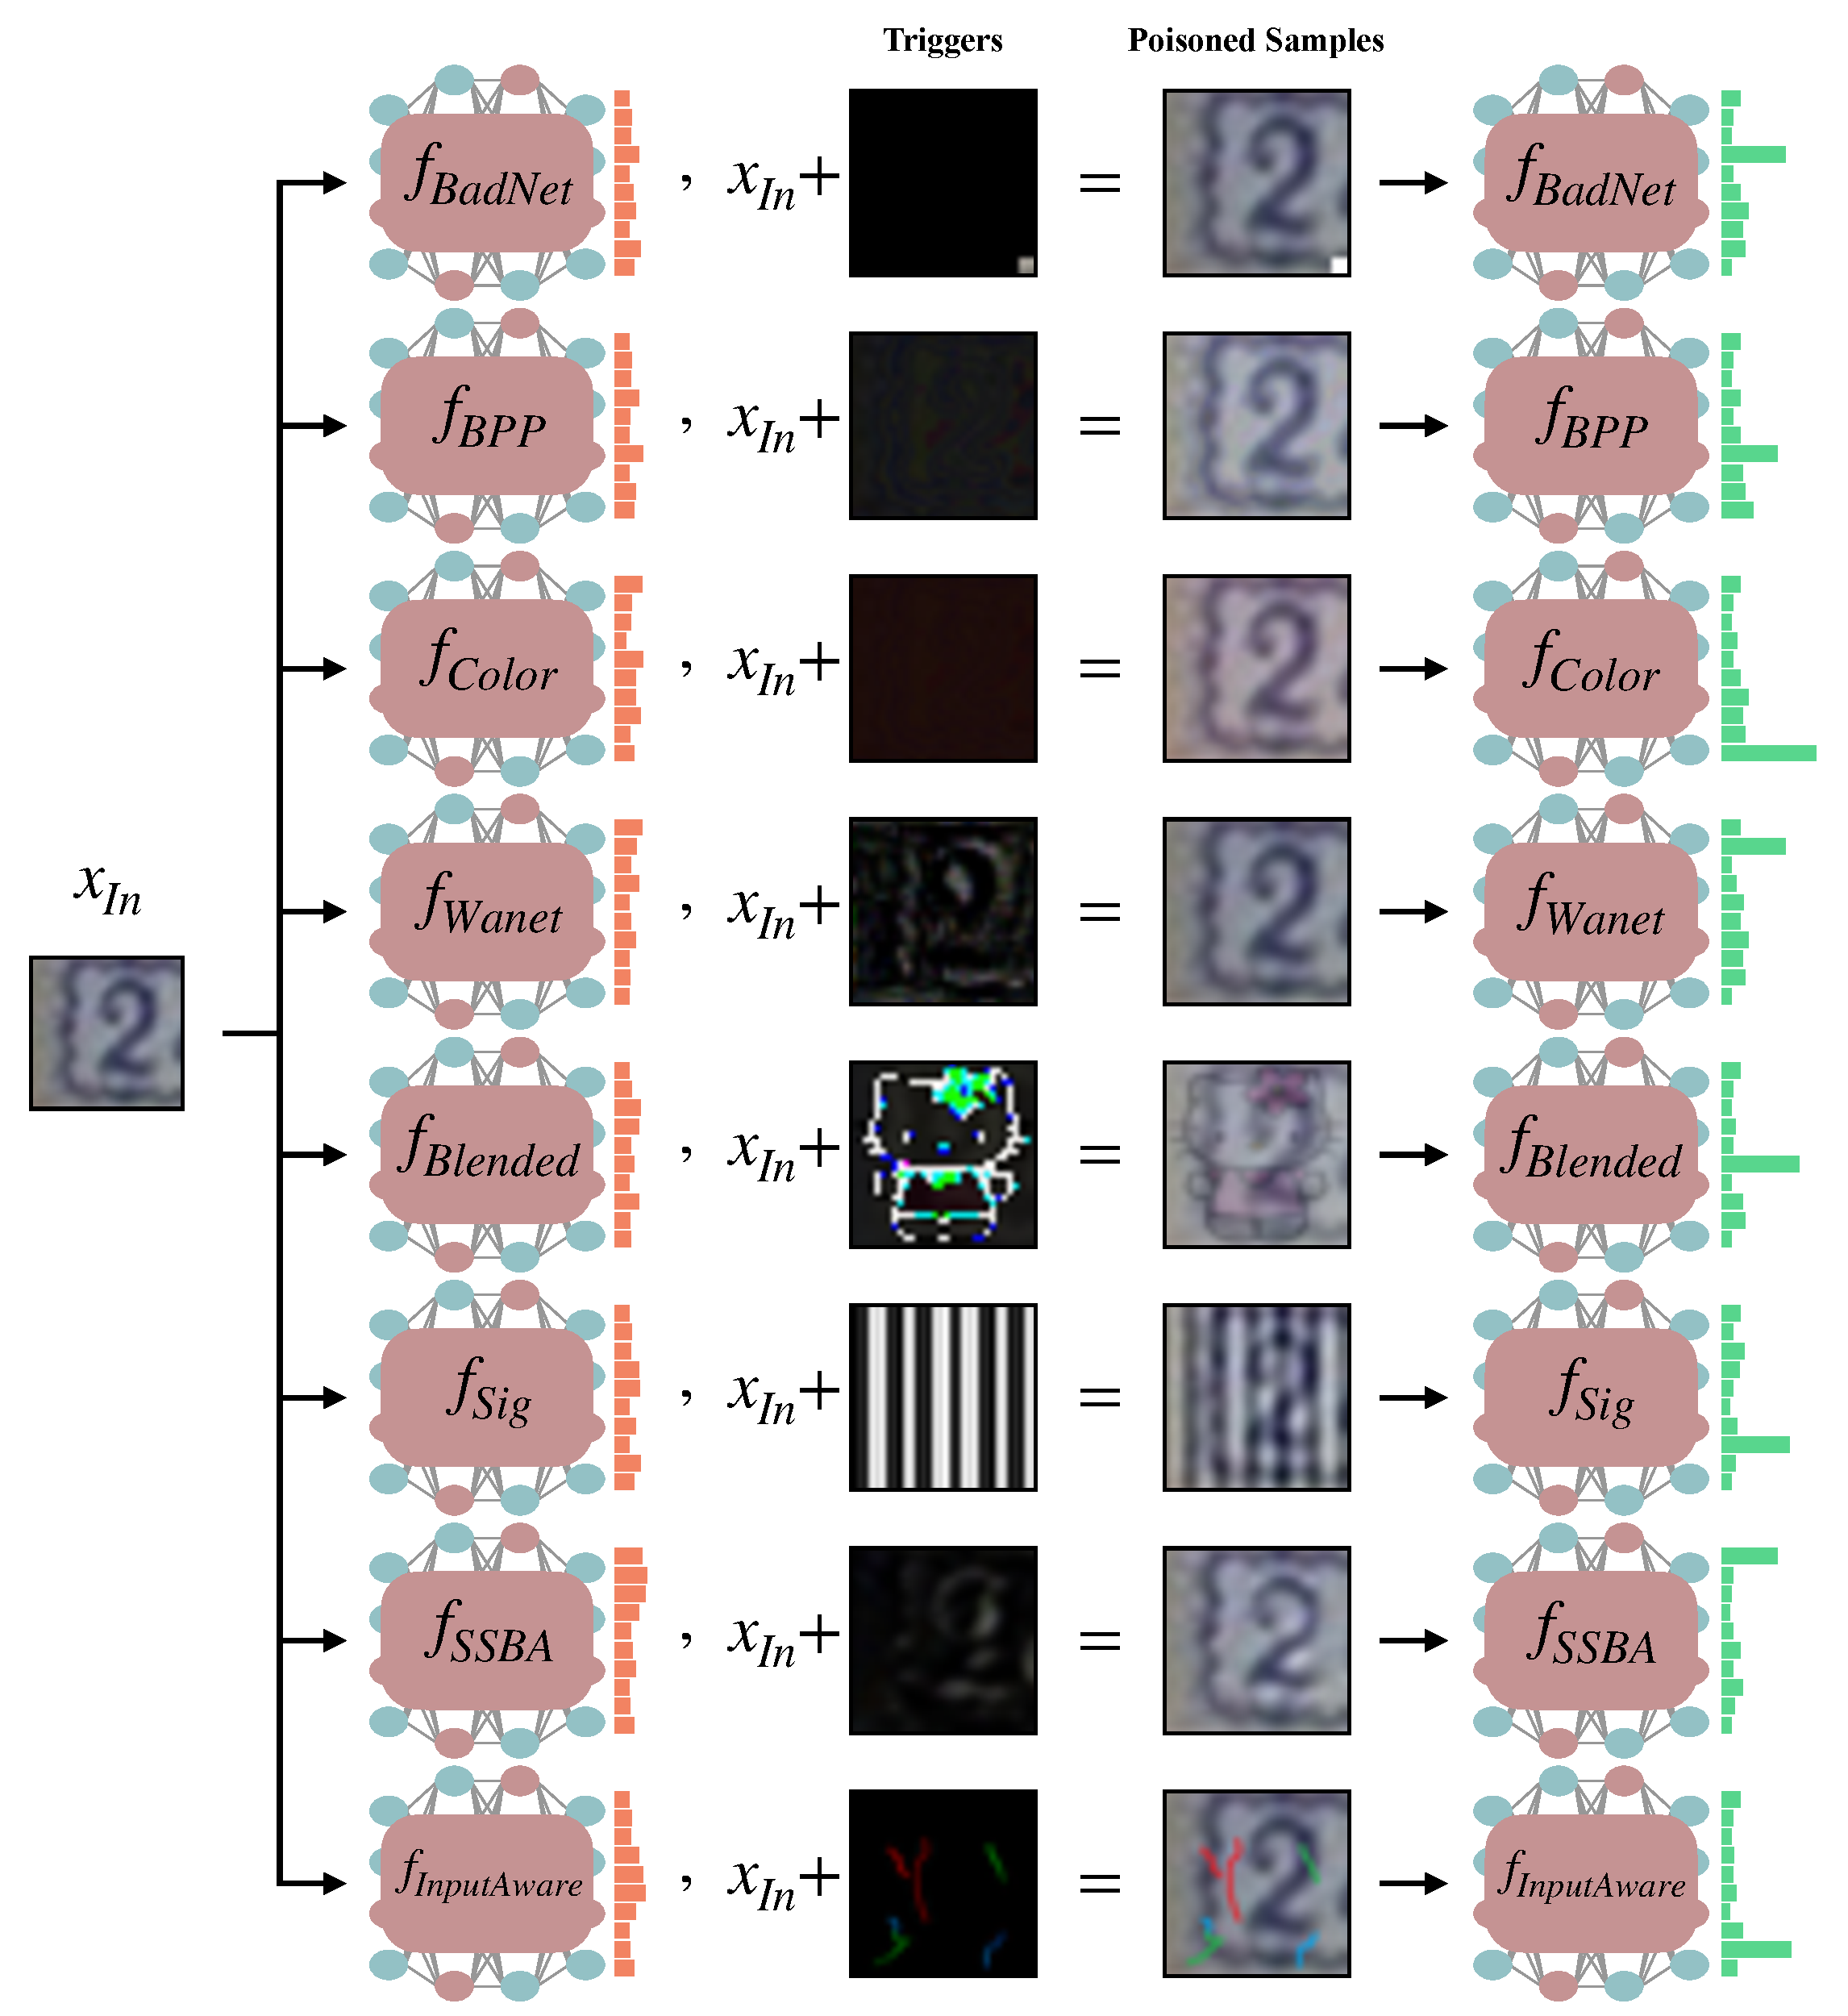
\includegraphics[width=1\linewidth]{Images/TriggerOnOOD.pdf}
    \caption{The effect of overlaying triggers on OOD data, in various attacks. As demonstrated, applying the trigger (which is used to poison training data) on even far-OOD samples, fools the model into identifying them as ID. This is due to the benign overfitting on the trigger present in the training data.}
    
    \vspace*{-4mm}
\label{TriggerOnOOD}

  \end{center}
\end{figure*}